% !TeX program = pdflatex
% =============================================================================
% Quiz: Magnetfelder (Multiple Choice)
% UZH Praktikum I -- 4fh, basierend auf arbeitsblatt5-magnetfelder.tex
% =============================================================================
\documentclass[11pt,a4paper]{article}

\usepackage[T1]{fontenc}
\usepackage[utf8]{inputenc}
\usepackage[ngerman]{babel}
\usepackage[a4paper,margin=2.2cm]{geometry}
\usepackage{amsmath}
\usepackage{graphicx}
\usepackage{enumitem}
\setlength{\parindent}{0pt}
\setlength{\parskip}{0.6em}

\begin{document}

\begin{center}
{\Large\bfseries Quiz: Magnetfelder (Multiple Choice)}
\end{center}
\noindent\textbf{Klasse:} 4fh \hfill \textbf{Thema:} Magnetfelder \hfill \textbf{Basis:} Arbeitsblatt 5

\bigskip
Wählen Sie pro Frage die eine richtige Antwort aus (A bis D).

\bigskip

\textbf{Frage 1}\\
Was ist ein Magnetfeld?
\begin{enumerate}[label=\Alph*)]
  \item Eine physikalische Kraft, die nur zwischen zwei Permanentmagneten wirkt
  \item Ein Modell für den Raum, in dem magnetische Wirkungen auftreten
  \item Die Bezeichnung für den Nordpol eines Stabmagneten
  \item Eine Einheit zur Messung der Stärke eines Elektromagneten
\end{enumerate}

\textbf{Frage 2}\\
Welche der folgenden Aussagen über das Zeichnen von Magnetfeldlinien ist falsch?
\begin{enumerate}[label=\Alph*)]
  \item Feldlinien verlaufen ausserhalb des Magneten vom Nordpol zum Südpol
  \item Feldlinien können sich kreuzen, wenn zwei Magnete nahe beieinander liegen
  \item Je dichter die Feldlinien gezeichnet sind, desto stärker ist das Feld
  \item Jede Feldlinie ist eine geschlossene Kurve
\end{enumerate}

\textbf{Frage 3}\\
Die abgebildete Spule ist rechtsgewickelt und an eine Batterie angeschlossen,
wie im Bild gezeigt ($+$ links, $-$ rechts).
\begin{center}
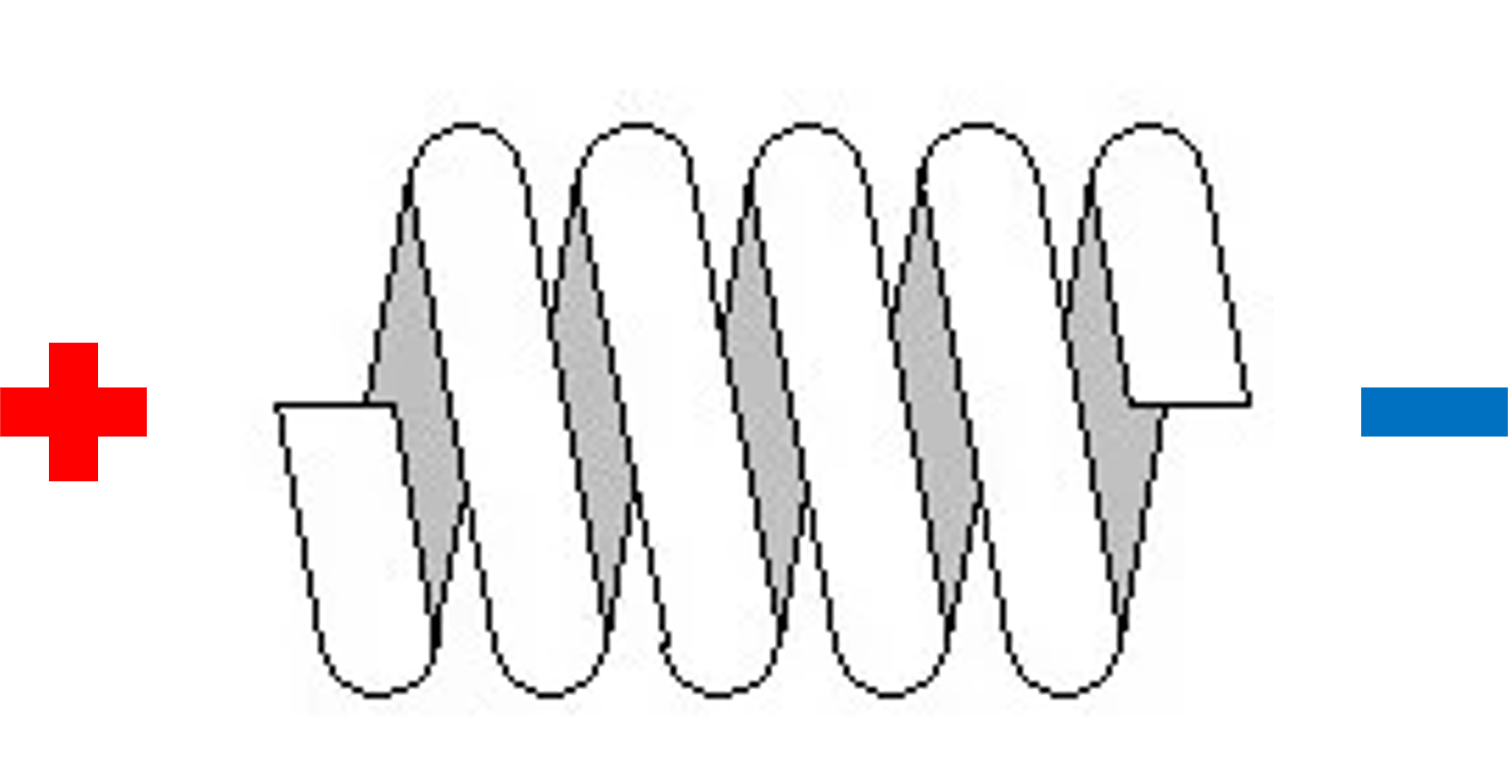
\includegraphics[width=7cm]{Bilder/windung_rechts.png}
\end{center}
Fahren Sie mit den gekrümmten Fingern der rechten Hand dem Draht in
Stromrichtung (von $+$ nach $-$) entlang. In welche Richtung zeigt der
Daumen, also das Magnetfeld im Innern der Spule?
\begin{enumerate}[label=\Alph*)]
  \item Nach links, Richtung Pluspol
  \item Nach rechts, Richtung Minuspol
  \item Senkrecht nach oben
  \item Senkrecht nach unten
\end{enumerate}

\textbf{Frage 4}\\
Für das Magnetfeld eines geraden, stromdurchflossenen Leiters gilt
$B = \dfrac{\mu_0}{2\pi}\cdot\dfrac{I}{r}$. Man verdreifacht den Strom $I$
und halbiert gleichzeitig den Abstand $r$ vom Draht. Was passiert mit $B$?
\begin{enumerate}[label=\Alph*)]
  \item $B$ verdoppelt sich
  \item $B$ verdreifacht sich
  \item $B$ versechsfacht sich
  \item $B$ bleibt gleich gross
\end{enumerate}

\textbf{Frage 5}\\
Die magnetische Flussdichte im Innern einer Spule ist gegeben durch
$B = \mu_0\cdot\dfrac{N}{l}\cdot I$. Zwei Spulen werden vom gleich grossen
Strom $I$ durchflossen: Spule A hat $N_A = 150$ Windungen bei einer Länge
$l_A = 25\,\text{cm}$, Spule B hat $N_B = 300$ Windungen bei einer Länge
$l_B = 60\,\text{cm}$. Welche Spule erzeugt die grössere Flussdichte $B$
im Innern?
\begin{enumerate}[label=\Alph*)]
  \item Spule A
  \item Spule B
  \item Beide Spulen erzeugen die gleiche Flussdichte
  \item Ohne den Wert von $I$ lässt sich das nicht bestimmen
\end{enumerate}

\bigskip
\hrule
\bigskip

\textbf{Antwortschlüssel}
\begin{enumerate}
  \item B. Ein Magnetfeld ist ein Modell für den Raum, in dem magnetische
  Wirkungen auftreten.
  \item B ist falsch: Feldlinien dürfen sich nie kreuzen oder berühren.
  \item B, nach rechts Richtung Minuspol: Die gekrümmten Finger folgen der
  rechtsgewickelten Spule von $+$ nach $-$, der Daumen zeigt dabei nach
  rechts.
  \item C, $B$ versechsfacht sich, da $B \propto I/r$. Die Verdreifachung
  von $I$ vergrössert $B$ um den Faktor $3$, die Halbierung von $r$
  vergrössert $B$ zusätzlich um den Faktor $2$. Beide Effekte wirken in
  dieselbe Richtung und multiplizieren sich: $3 \cdot 2 = 6$.
  \item A, Spule A erzeugt die grössere Flussdichte. Massgeblich ist die
  Windungsdichte $n = N/l$, nicht die Windungszahl $N$ allein:
  $n_A = 150 / 0{,}25\,\text{m} = 600\,\text{pro Meter}$ ist grösser als
  $n_B = 300 / 0{,}6\,\text{m} = 500\,\text{pro Meter}$. Da $B = \mu_0\cdot
  n\cdot I$ und $I$ bei beiden Spulen gleich gross ist, hat Spule A die
  grössere Flussdichte.
\end{enumerate}

\end{document}
